\documentclass{article}%
\usepackage[T1]{fontenc}%
\usepackage[utf8]{inputenc}%
\usepackage{lmodern}%
\usepackage{textcomp}%
\usepackage{lastpage}%
\usepackage{authblk}%
\usepackage{graphicx}%
%
\title{Preparation of Monoclonal Antibodies Cross{-}Reactive with Orthopoxviruses and Their Application for Direct Immunofluorescence Test}%
\author{Victoria Armstrong}%
\affil{Blood Transfusion Centre of Slovenia, Ljubljana, Slovenia}%
\date{01{-}01{-}2014}%
%
\begin{document}%
\normalsize%
\maketitle%
\section{Abstract}%
\label{sec:Abstract}%
With the poster from IDB on display here.\newline%
According to research published in the Journal of the National Cancer Institute, levels of a key cytokine in the blood of breast cancer patients are changing after treatment for the disease.\newline%
In the study, mice that had undergone inoperable or metastatic breast cancer and received phosphorylation of a particular receptor surface molecule (PsMA) after they received chemotherapy responded to platinum{-}based chemotherapy, thus strengthening the reduction of the progression{-}free survival as measured by the NWCRP Protein Density Score.\newline%
The results also indicated that in these mice, attacks were less advanced as compared to in patients treated with platinum{-}based chemotherapy alone, and those treated with gemcitabine did not show evidence of the phosphorylation of the receptor surface molecule.\newline%
In fact, when evaluated against the overall progression{-}free survival (PFS) scores of the patients receiving platinum{-}based chemotherapy alone, the first three months of survival time improved a minimum of 21 percent. The researchers also observed reductions in breast tissue and lymphocytes more generally.\newline%
This is an important signal of where to go with the whole picture of the tumor, explained Michael Miller, M.D., M.P.H., an immunologist at the Dana{-}Farber Cancer Institute and The Dana{-}Farber Cancer Institute.\newline%
In the studies, the results were significant enough that the lead investigators decided to test further their potential predictive value against other regulatory factors involved in the control of disease progression.

%
\subsection{Image Analysis}%
\label{subsec:ImageAnalysis}%


\begin{figure}[h!]%
\centering%
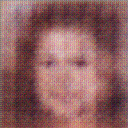
\includegraphics[width=150px]{500_fake_images/samples_5_63.png}%
\caption{A Man With A Beard Wearing A Tie}%
\end{figure}

%
\end{document}